% --------------------------------------------------------------
% Abhi's Standard math Preamble.
% --------------------------------------------------------------
 
% Document packages / layout
\documentclass[12pt]{article}
\usepackage[margin=1in]{geometry} %1 inch margins

% Figure Packages
\usepackage{float}
\usepackage[plainpages=false, colorlinks=true, allcolors=cyan]{hyperref}
\usepackage{url}
\usepackage{subcaption}
\usepackage{wrapfig}
\usepackage[export]{adjustbox} %center option in include graphics
\usepackage[splitrule]{footmisc}
%\interfootnotelinepenalty=10000

% Math Packages
\usepackage{amsmath,amsthm,amssymb,mathrsfs,bm}
\usepackage{mathtools}
\usepackage{commath}
\usepackage{esvect} %For derivatives of vectors \vec{u}' -> \vv{u}'

% Code input 
\usepackage{algorithm}
\usepackage{algpseudocode}
%Manual indentation 
\algdef{SE}[SUBALG]{Indent}{EndIndent}{}{\algorithmicend\ }%
\algtext*{Indent}
\algtext*{EndIndent}
\makeatletter
\newenvironment{breakablealgorithm}
  {% \begin{breakablealgorithm}
   \begin{center}
     \refstepcounter{algorithm}% New algorithm
     \hrule height.8pt depth0pt \kern2pt% \@fs@pre for \@fs@ruled
     \renewcommand{\caption}[2][\relax]{% Make a new \caption
       {\raggedright\textbf{\ALG@name~\thealgorithm} ##2\par}%
       \ifx\relax##1\relax % #1 is \relax
         \addcontentsline{loa}{algorithm}{\protect\numberline{\thealgorithm}##2}%
       \else % #1 is not \relax
         \addcontentsline{loa}{algorithm}{\protect\numberline{\thealgorithm}##1}%
       \fi
       \kern2pt\hrule\kern2pt
     }
  }{% \end{breakablealgorithm}
     \kern2pt\hrule\relax% \@fs@post for \@fs@ruled
   \end{center}
  }
\makeatother

% Quality of Life Packages
\usepackage{enumerate}
\usepackage{cite}

\newcommand{\hogwild}{H{\sc ogwild}!}
\newcommand{\E}[1]{\mathbb{E}\left[#1\right]}
\newcommand{\Prob}[1]{\mathbb{P}\left[#1\right]}
\newcommand{\Var}[1]{{\rm Var}\left[#1\right]}

\newcommand{\e}{\varepsilon}

\newtheorem{theorem}{Theorem}[section]
\newtheorem{lemma}{Lemma}[section]
\newtheorem{definition}{Definition}[section]
 
\begin{document}
 
\title{An Investigation into \hogwild%
\footnote{
  See \url{https://github.com/abhijit-c/HOGWILD}.
}
}
\author{%
  Abhijit Chowdhary \\
  \texttt{ac6361@nyu.edu}
}
\date{New York University --- \today}

\maketitle

\addtocontents{toc}{~\hfill\textbf{Page}\par} % Add 'page' above pg numbers
\tableofcontents
\clearpage

\section{Introduction}

Despite being the subject of much modern excitement, the ideas of gradient
descent date all the way back to Cauchy in 1847. And although it's main
application has been in the solution of recent big-data optimization problems,
stochastic gradient has been around since the 1940s, formally by Robbins and
Monro in 1951. In the last two decades, however, modern hardware has begun to
see a tapering off of Moore's law, and has begun to expand out in a distributed
fashion with multicore processors and GPUs; naturally the question becomes: In
order to take advantage of the strengths of modern hardware, how can we
parallelize a stochastic gradient method?

\section{\hogwild}

Prior to 2011, parallel stochastic gradient methods had been introduced, but
most suffered from poor scaling due to the necessity of locks. A naive
implementation could look like:
\begin{breakablealgorithm}
  \caption{Very Naive Parallel Stochastic Gradient}
  \label{alg:naivePSG}
  \begin{algorithmic}[1]
    \Require Number of data points $N$, seperable loss function $f
    = \sum_{e \in E} f_e(x_e)$, Initial $x$.
    \For{epoch $= 0 \to$ MAX\_EPOCHS}
      \State \#pragma omp parallel for
      \For{$k = 0 \to N$}
        \State Choose $i$ uniformly from $\{1, \dots, |E|\}$.
        \State \#pragma omp critical
        \Indent
          \State Read current parameters $x$.
          \State Compute $\nabla f_i(x)$.
          \State $x \gets x - \eta \nabla f_i(x)$.
        \EndIndent
      \EndFor
    \EndFor
  \end{algorithmic}
\end{breakablealgorithm}
But it's clear here that such an algorithm would only effectively be
parallelizing the unform sample of $i$ in $\{1, \dots, |E|\}$. You can improve
the above by selectively locking the values in $x$ which actually change in the
stochastic gradient step (say if $\nabla f_i(x)$ was sparse), but because the
process of acquiring locks is much more expensive than floating point
arithmetic, this helps little.

However, in 2011, the article "\hogwild: A Lock-Free Approach to Parallelizing
Stochastic Gradient Descent" proposed a very simple solution to this problem.
Remove the locks!
\begin{breakablealgorithm}
  \caption{Very Naive Parallel Stochastic Gradient}
  \label{alg:naivePSG}
  \begin{algorithmic}[1]
    \Require Number of data points $N$, seperable loss function $f
    = \sum_{e \in E} f_e(x_e)$, Initial $x$.
    \For{epoch $= 0 \to$ MAX\_EPOCHS}
      \State \#pragma omp parallel for
      \For{$k = 0 \to N$}
        \State Choose $i$ uniformly from $\{1, \dots, |E|\}$.
        \State Read current parameters $x$.
        \State Compute $\nabla f_i(x)$.
        \State $x \gets x - \eta \nabla f_i(x)$.
      \EndFor
    \EndFor
  \end{algorithmic}
\end{breakablealgorithm}
 
\section{Convergence Analysis}
a
\subsection{Theoretical Results}
\subsection{Numerical Validation}
\begin{figure}[!htb]
  \centering
  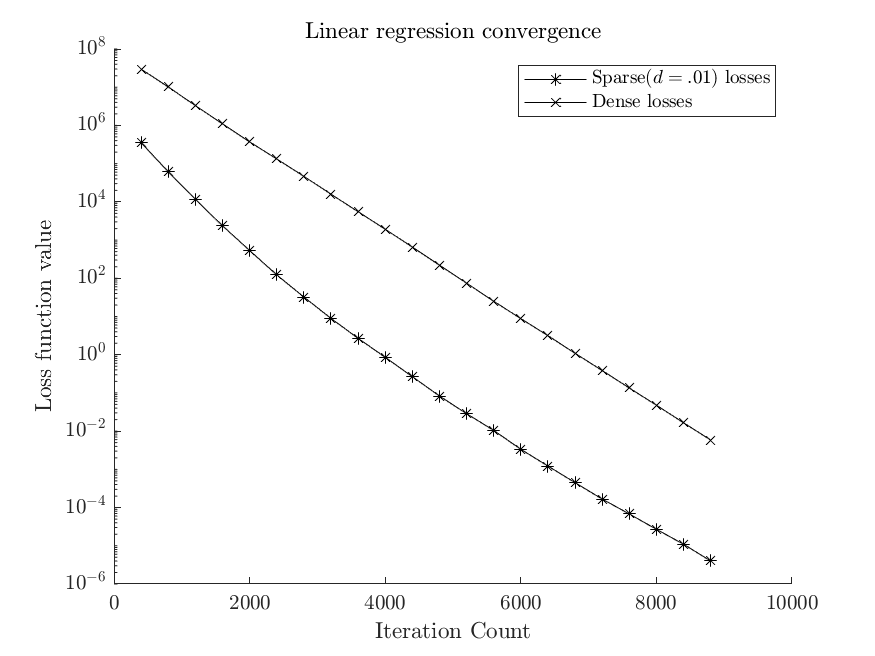
\includegraphics[width=.8\textwidth]{./resources/convergence}
\end{figure}

\section{Efficiency Analysis}

\subsection{Theoretical Results}

\subsection{Numerical Validation}
\begin{figure}[!htb]
  \centering
  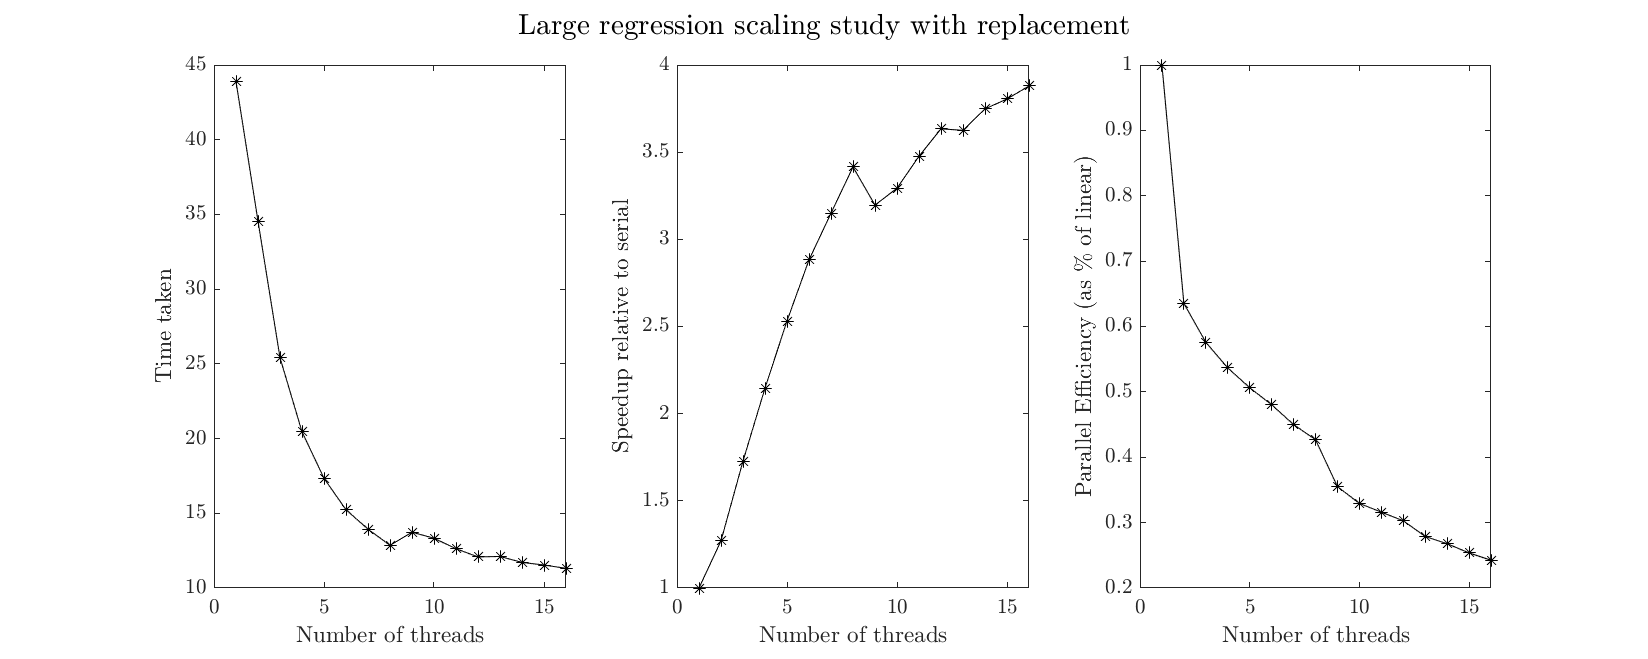
\includegraphics[width=1\textwidth]{./resources/replacement}
\end{figure}
\begin{figure}[!htb]
  \centering
  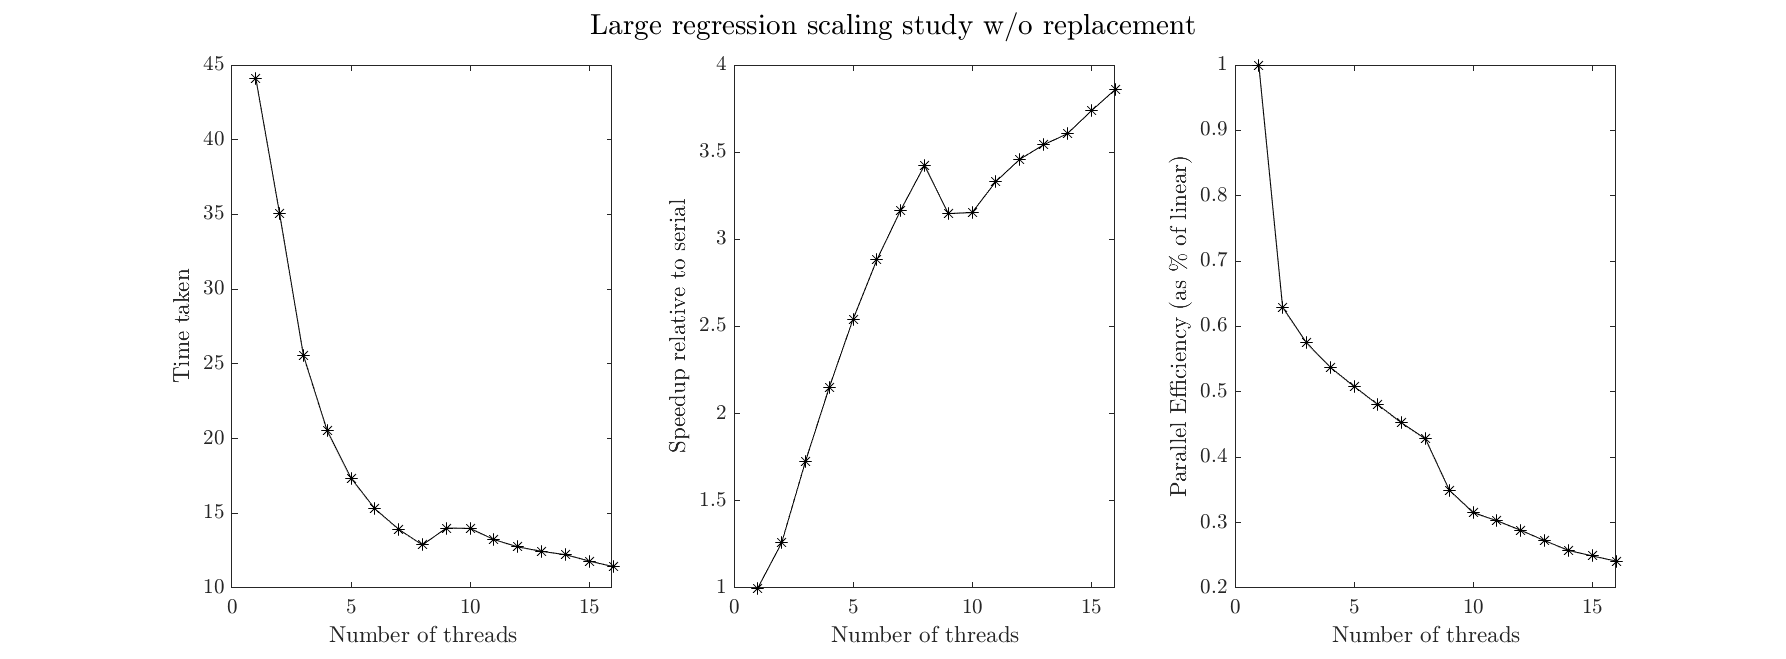
\includegraphics[width=1\textwidth]{./resources/noreplacement}
\end{figure}
\begin{figure}[!htb]
  \centering
  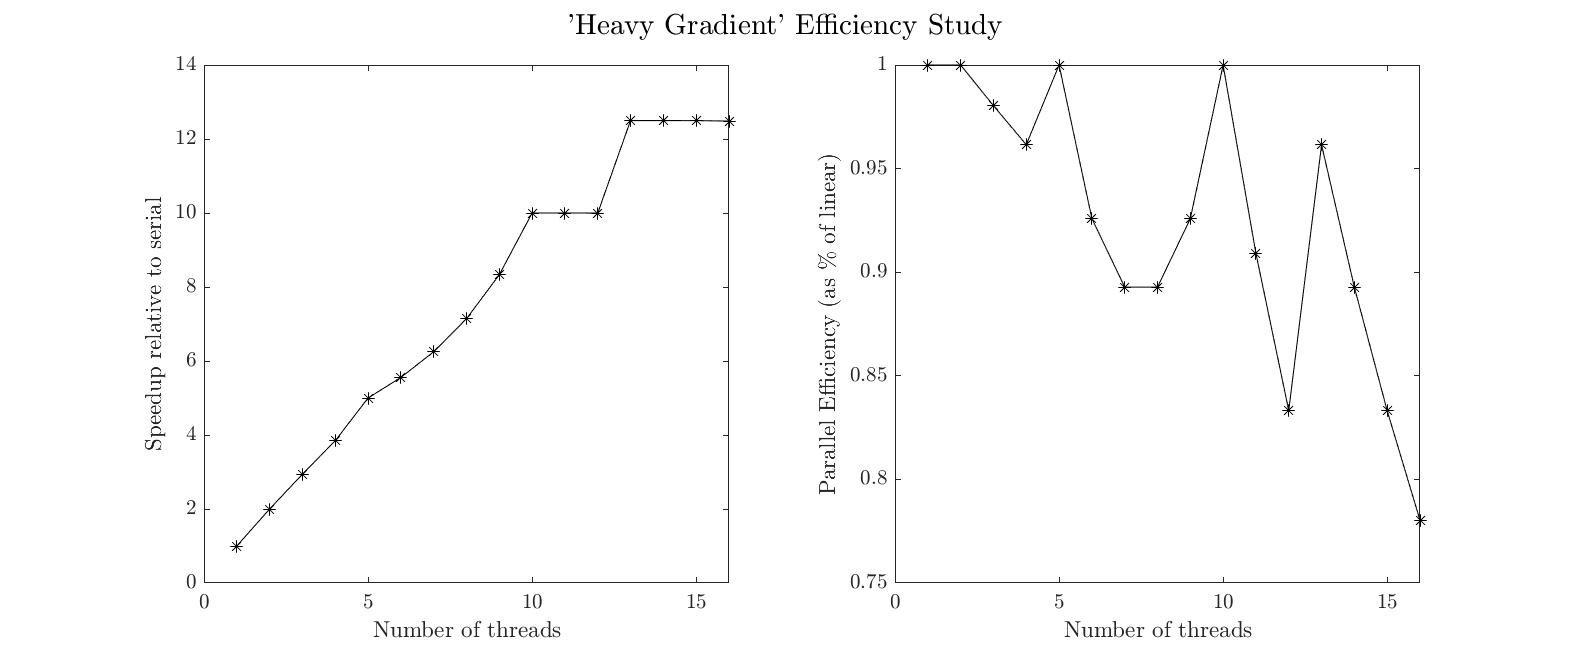
\includegraphics[width=\textwidth]{./resources/heavy_gradient}
\end{figure}

\section{Applications: Judging Wine Quality}

As a sort of fun application, I found a dataset on UCI's archive from a paper by
Cortez et al. \cite{2009CCAMR} which charted various physicochemical properties
of a set of white wine, and had corresponding 'quality' (judged by a committee,
the CVRVV) levels for each data point. The reason why I decided to try this
dataset, is not only because knowing what makes alcohol quality clearly
a very important task, but also because in the original paper, their uncertainty
regarding the relevancy of all input variables was noted. That is, this is an
interesting opportunity to try a feature selection method: my method of choice
this time was ridge-regression, the $\ell^2$ variant of LASSO. See Figures
\ref{fig:linearwine} and \ref{fig:ridgewine} for the linear and ridge regression
variants, respectively.
\begin{figure}[!htb]
  \centering
  \begin{subfigure}{.5\textwidth}
    \centering
    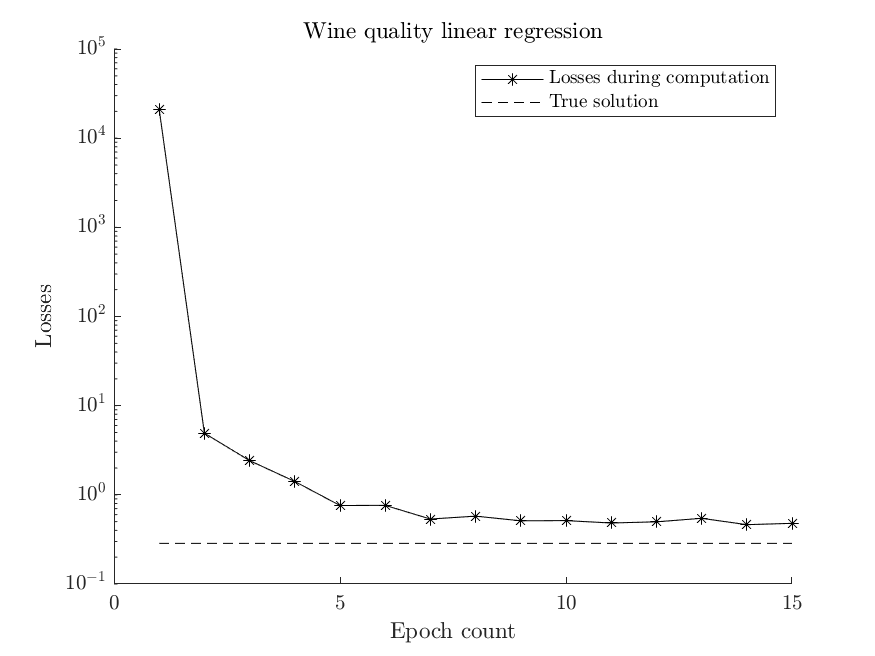
\includegraphics[width=\linewidth]{./resources/linear_wine}
    \caption{}\label{fig:linearwine}
  \end{subfigure}%
  \begin{subfigure}{.5\textwidth}
    \centering
    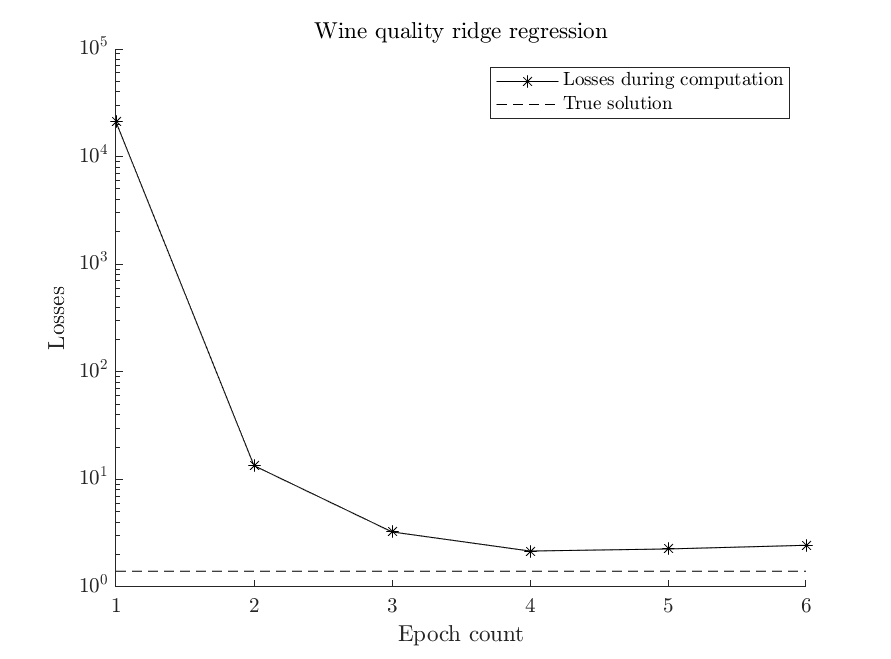
\includegraphics[width=\linewidth]{./resources/ridge_wine}
    \caption{}\label{fig:ridgewine}
  \end{subfigure}
  \caption{
    Both converge in rougly four to eight epochs, but it should be noted
    that neither converges to the true solution. Regardless of how I chose the
    learning rate, it appeared that both runs of \hogwild\ would get stuck in
    a noise ball somewhere close to the true solution. This is an important
    failing of stochastic gradient methods in general, sometimes the noise
    generated will prevent us from seeing a 'true' solution, and indeed the
    ridge-regressed version didn't properly feature select, whereas the solution
    computed via CVX saw the 11th feature to be most weighted (The 11th feature,
    to my amusement, is alcohol content. Certainly an important part of what
    makes a good wine...).
  }
\end{figure}

\section{Conclusions and Future Work}\label{sec:conclusion}


\clearpage
\addcontentsline{toc}{section}{Works Cited}
\bibliography{references}{}
\bibliographystyle{alpha}

\end{document}
